\documentclass[runningheads]{llncs}

\usepackage{graphicx}
\usepackage{booktabs}
\usepackage{amsmath}
\usepackage{url}

\graphicspath{{../results/}}

\begin{document}

\title{Size-Specific Expert Segmentation and Boundary-Band Policy Refinement for Brain Tumor MRI}
\titlerunning{Boundary-Band Policy Refinement for Brain Tumor MRI}

\author{Inseong Ahn\inst{1} \and Sujin Han\inst{2}}
\authorrunning{Ahn and Han}
\institute{Department of Computer Engineering, Gachon University, Seongnam, Korea
\and
Department of Artificial Intelligence, Gachon University, Seongnam, Korea}

\maketitle

\begin{abstract}
Whole-tumor regions on brain MRI vary in cross-sectional size and boundary appearance, so a single segmentation model is a poor fit for every scale. We classify tumor size on $128\times128$ axial slices from T1ce and FLAIR, build an initial mask with a size-specific expert, and then let one class-shared PPO turn pixels on or off inside a fixed band. Slices below 300 pixels use a 2.5D CaraNet, slices from 300 up to 700 use UNet++, and slices of 700 pixels or more use a SegResNet that predicts edema and tumor core separately. A single refinement policy edits pixels whose expert probability lies in $[0.35,0.65]$ or that lie within $\pm2$ pixels of the mask boundary. Ground truth enters only the training reward, not the inference observation. A FLAIR relative-intensity constraint is applied only to the action at the last step.

We evaluate on 50{,}010 tumor slices from 851 of the 1{,}251 BraTS 2021 patients, after holding out a development set of 400 (280 train, 60 validation, 60 method selection). The metric is the patient mean of slice Dice similarity coefficients (DSC). Against a Stage~2 mask whose classifier routes each slice to an expert and whose thresholds are fixed at 0.80/0.80/0.50, DSC rises from 0.8337 to 0.8604 (paired patient difference $+0.0267$, 95\% CI $0.0256$--$0.0278$). The gain remains $+0.0193$ (95\% CI $0.0184$--$0.0202$) against a Stage~2 variant whose per-size thresholds were reselected on the 60 validation patients (DSC 0.8411). The change from 0.8337 to 0.8604 uses weights locked on 2026-09-30. Retraining the same split on 2026-10-07 at seeds 42, 7, and 123 gives boundary-band PPO patient-mean DSC of 0.8597, 0.8620, and 0.8609 (range 0.0023). At seed 42 the empty-slice false-positive rate is 0.521, Dice after stacking slices into a volume is 0.813, and the patient-mean HD95 on slices where both masks are nonempty is 10.73\,mm. A single U-Net scores 0.8156; attaching a global shrink/keep/expand vanilla PPO scores 0.8133. These numbers are not BraTS 3D leaderboard scores. Code and experiment records are available at \url{https://github.com/aninsung/2026-summer-Interdepartmental-Academic-Conference}.

\keywords{Brain tumor segmentation \and Magnetic resonance imaging \and Reinforcement learning \and PPO \and Dynamic routing \and Boundary refinement}
\end{abstract}

\section{Introduction}

Tumor-region segmentation is used to quantify tumor burden and to define the treatment volume. On MRI, size, contrast pattern, and edema boundary change across patients and across slices of the same patient, so one backbone struggles to fit both tiny and large cross-sections. U-Net-style networks are the standard architecture for medical image segmentation~\cite{ronneberger2015}, but when the error pattern depends on size, the initial mask can retain a systematic under-segmentation along the boundary. In precision radiotherapy a small boundary error changes the treated volume, and correcting every slice by hand is slow.

This work separates initial segmentation from boundary refinement. A classifier selects the slice size, the corresponding expert produces a probability map, and one PPO edits only the ambiguous probability range and the neighborhood of the mask boundary. Because the policy does not redraw the whole mask, the interior that the expert already got right is kept, and the pixels it may change are confined to a band. The observation contains no ground truth; ground truth is used only in the training reward.

We call this three-stage pipeline TRIO: size classification, size-specific experts, and one boundary-band PPO. The contributions are:
\begin{enumerate}
\item a routed segmentation that builds the initial whole-tumor mask with small, medium, and large experts;
\item a single PPO, shared across sizes, that learns only to turn boundary-band pixels off, leave them, or turn them on.
\end{enumerate}
The band network trained by supervision on medium slices only is the initial weight of this PPO. That supervised correction, and any later supervised fine-tuning of the same network, is not a contribution. Fixing the metric definition and the evaluation set in advance is the experimental procedure, not a contribution.

\section{Related Work}

U-Net uses skip connections so that encoder localization and decoder semantics are available together, and it is the base architecture for medical image segmentation~\cite{ronneberger2015}. We place three models from this family on different size ranges.

\subsection{CaraNet}
CaraNet is a medical segmentation network designed to find very small objects~\cite{lou2023}. A context module sits on the encoder features, and a block that combines axial attention and reverse attention shifts attention to the outside of the region already found, where the boundary is easy to miss. Supervision is applied to outputs at several stages. We use it as the small expert, for areas below 300 pixels.

\subsection{SegResNet}
SegResNet is an encoder--decoder that inserts ResNet residual blocks~\cite{myronenko2018}. Each block applies normalization, ReLU, and convolution twice and then adds the input. The original model segments 3D brain-tumor MRI and attaches a reconstruction branch from the encoder output as a regularizer. We use it as the large expert, for areas of 700 pixels or more, and merge separate edema and tumor-core predictions into a whole-tumor probability.

\subsection{UNet++}
UNet++ connects encoder and decoder with nested dense skip connections~\cite{zhou2019}. Features at the same resolution pass through intermediate nodes, which reduces the semantic gap between encoder and decoder features and improves boundary accuracy. Deep supervision can be applied to outputs of several depths. We use it as the medium expert, for areas from 300 up to 700 pixels.

\subsection{PPO}
Proximal policy optimization (PPO) is a policy-gradient reinforcement-learning algorithm~\cite{schulman2017}. Sampling, in which the agent observes a state, chooses an action, and receives a reward, alternates with training, in which the collected trajectories yield a loss that updates the policy network. Clipping the probability ratio between the new and old policies limits the size of one update and stabilizes learning. Reusing the same trajectories for several epochs spends samples more efficiently than a plain policy gradient. Here one slice is the environment, and the action at each band pixel is off, keep, or on.

In medical imaging, multi-agent iterative refinement of 3D boundaries~\cite{liao2020} and pixel-level reinforcement learning~\cite{furuta2020} have been reported. nnU-Net is a self-configuring segmentation method that selects preprocessing and model choices from the data~\cite{isensee2021}. The multi-institutional MRI and expert labels of BraTS were organized by Menze et al.~\cite{menze2015} and Bakas et al.~\cite{bakas2017}; the scans in this study are the 2021 task in that line~\cite{baid2021}. Unlike cascade methods that narrow a coarse mask and then redraw the boundary~\cite{wang2018,chen2016}, this work edits only a prescribed band of a size-specific expert mask. Our policy is not split by size. Its action is not a parallel shift of the contour by one value; it changes pixel labels inside a prescribed band. During development we also examined per-direction distance shifts and closed-contour regression, but the adopted implementation is boundary-band refinement. Those development numbers are the method-selection record in Section~\ref{sec:select}, and the locked performance is Section~\ref{sec:locked}.

\section{Method}
\label{sec:method}

Figure~\ref{fig:pipeline} is the full pipeline. The classifier chooses the slice size, a size-specific expert builds the initial mask, and the boundary-band PPO edits only pixels inside the band.

\begin{figure}[t]
\centering
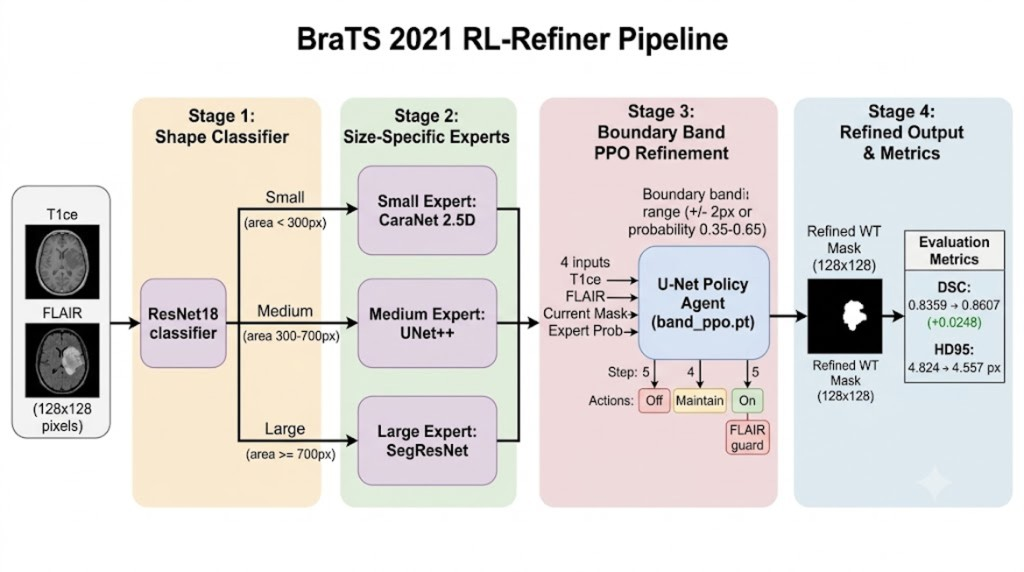
\includegraphics[width=\textwidth]{pipeline_overview.jpg}
\caption{Pipeline. Stage~1 classifies size, Stage~2 runs a size-specific expert, Stage~3 applies the boundary-band PPO, and Stage~4 evaluates.}
\label{fig:pipeline}
\end{figure}

\subsection{Data and Split}
The inputs are T1ce and FLAIR from BraTS 2021~\cite{baid2021}. Slices are resized to $128\times128$, z-score normalized inside the brain, clipped to the 1st--99th percentiles, and scaled to $[0,1]$. Only slices whose tumor-pixel fraction is at least 0.2\% enter training and evaluation. Whole tumor is every pixel whose segmentation label is nonzero. Size is defined by the ground-truth area: below 300 pixels is small, from 300 up to 700 is medium, and 700 or more is large.

Splits are by patient, so adjacent slices of the same patient do not fall into both training and validation. Of 1{,}251 patients, a development set of 400 drawn with seed 42 is split into 280 train, 60 validation, and 60 method selection. The remaining 851 patients (50{,}010 tumor slices) were not used to train weights or to select the method in this study. The fixed Stage~2 thresholds 0.80/0.80/0.50 and the connected-component sizes do come from an earlier protocol (a 210-patient pool drawn with the same seed), and 148 patients from that pool are among these 851. The band design was chosen on the current method-selection set of 60. Table~\ref{tab:split} lists these roles.

\begin{table}[t]
\caption{Patient split.}
\label{tab:split}
\centering
\begin{tabular}{lrl}
\toprule
Role & Patients & Use \\
\midrule
Train & 280 & Classifier, experts, boundary-band PPO \\
Validation & 60 & Checkpoint selection; baseline thresholds \\
Method selection & 60 & Policy adoption. Not the reported performance \\
Locked evaluation & 851 & Patient mean from a single application \\
\bottomrule
\end{tabular}
\end{table}

\subsection{Routing and Experts}
The classifier is a ResNet-18 initialized from ImageNet. Its input is 2.5D, formed by stacking neighboring slices, and the first convolution is adapted by summing the RGB kernel along the channel axis. Slices within $\pm80$ pixels of an area boundary are dropped from classifier training to reduce label noise at the cut points. The loss is cross-entropy with label smoothing 0.05. Validation accuracy for this run is 0.8151. On the 851-patient slices, the classifier matches the ground-truth size on a fraction 0.801 of slices.

At inference the classifier selects the expert. Below 300 pixels the expert is a 2.5D CaraNet: six input channels, oversampling of very small ground-truth masks, and a second pass after cropping to $64\times64$. From 300 up to 700 pixels the expert is a UNet++ on the two channels of the center slice. At 700 pixels or more, SegResNet predicts edema and tumor core separately and merges them as $1-(1-p_{\mathrm{ED}})(1-p_{\mathrm{TC}})$. The large expert is trained on all sizes and, at inference, is used only on slices classified as large.

Probabilities are the mean of the original and of horizontal and vertical flips. Binarization thresholds are 0.80, 0.80, and 0.50 for small, medium, and large, and the minimum connected-component sizes are 0, 15, and 25 pixels. These thresholds were kept from the earlier protocol and were not reselected on the current development validation; the control that reselects them on the 60 validation patients is Section~\ref{sec:retune}. Experts train for 20 epochs, batch size 64, Adam with learning rate $3\times10^{-4}$, a cosine schedule, and mixed precision. The loss is the sum of binary cross-entropy and Dice. On this split the small CaraNet has validation DSC 0.8159.

Expert selection during training differs from inference. Policy training and checkpoint selection route by ground-truth area. On 19.9\% of the 851 evaluation slices, the policy refines a mask from an expert other than the one that was trained for that ground-truth size.

\subsection{Boundary-Band PPO}
\begin{figure}[t]
\centering
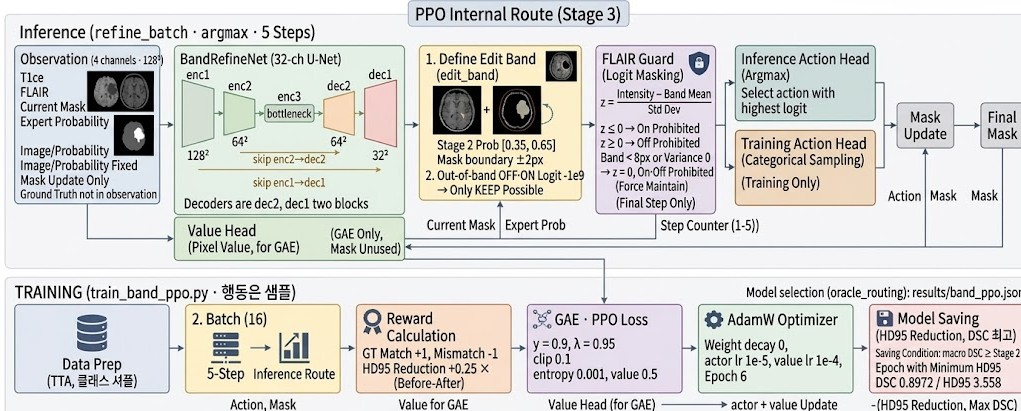
\includegraphics[width=\textwidth]{fig2_ppo_internal_route.jpg}
\caption{Internal route of the boundary-band PPO. The upper path is five-step argmax inference. The lower path is training: reward, GAE--PPO loss, and the AdamW update of the action and value heads. Locked numbers are in Table~\ref{tab:locked}.}
\label{fig:ppo-route}
\end{figure}
There is one policy. Its initialization is a band-refinement network trained by supervision on medium slices only. That supervised correction is initialization, not a contribution. The contributions are size-specific routing and the PPO that edits the band of that mask. Supervised fine-tuning of the same network on all sizes is also not a contribution. The network is a small U-Net of width 32. The four input channels are T1ce, FLAIR, the current mask, and the expert probability. Ground truth is not an observation. At the end of the decoder an action head and a value head split. The action head emits three logits per pixel (off, keep, on), and inference takes the argmax. The value head is used only in training. Outside the band, the off and on logits are masked so the action is keep.

Editable pixels are those whose expert probability is in $[0.35,0.65]$, or those within 2 pixels of the current mask boundary. Outside the band the Stage~2 label is kept. A pixel inside the probability interval can change even if it is far from the boundary, so the editable set is not only the $\pm2$-pixel rim. Over five steps the probability map stays fixed and only the mask is passed to the next observation.

The FLAIR constraint applies only to the last step. Relative intensity is computed from the mean and standard deviation of the band on that slice: pixels darker than the mean cannot be turned on at the last step, and brighter pixels cannot be turned off. If the band has fewer than 8 pixels or has no variance, the slice keeps the Stage~2 mask. Steps 1--4 have no such constraint, so a pixel turned on earlier is not always reversed at the last step. The final mask is not assumed to satisfy the FLAIR rule. Slices whose DSC falls are not reverted to the initial mask.

The reward uses ground truth only during training. A flipped pixel scores $+1$ if it matches the ground truth and $-1$ otherwise. When both masks are nonempty so that HD95 can be computed, the HD95 decrease multiplied by 0.25 is added at every flipped pixel. The HD95 term therefore scales with the number of flips. Generalized advantage estimation (GAE) is computed on band pixels only. The PPO clip is 0.1, the discount is 0.9, GAE $\lambda$ is 0.95, the entropy coefficient is 0.001, and the value coefficient is 0.5. The optimizer is AdamW, with action learning rate $1\times10^{-5}$ and value learning rate $1\times10^{-4}$. Training runs for 6 epochs, with 2 PPO epochs and batch size 16. The three size classes are mixed in one batch.

The saved epoch is the one whose macro DSC under ground-truth-area routing is at least that of Stage~2 and whose macro HD95 is the lowest. The saved model is epoch 5, with validation macro DSC 0.8972 and HD95 3.558. Stage~2 on the same validation set has DSC 0.8741 and HD95 3.838.

Figure~\ref{fig:ppo-route} is the internal route. Inference takes the four-channel observation, defines the edit band, applies the FLAIR guard only at the last step, and updates the mask for five steps by argmax. Training uses ground truth only in the reward. A batch of 16 runs the five-step route, and GAE--PPO updates the action and value heads.

\subsection{Metrics}
The primary metric is the patient mean of slice DSC. Slices within a patient are averaged with equal weight, and patients are averaged with equal weight. Slices with tumor-pixel fraction below 0.2\% are excluded. This is not the BraTS 3D volume Dice. Comparisons with Stage~2 use the interval of the paired patient difference, the 2.5--97.5 percentiles of 2{,}000 patient-level bootstrap resamples.

HD95 is the 95\% surface distance between the two contours on the same $128\times128$ grid, in pixels, not millimetres. If either the prediction or the ground truth is empty, that slice is dropped from the HD95 mean, and the dropped slices can differ between methods. Equal patient counts therefore do not make this a paired comparison on the same slice set, and we do not use it as a claim. HD95 values in the tables are descriptive means under this definition.

Size rows are not patient cohorts. Each row pools slices whose ground-truth area falls in that range and then averages patients who have at least one such slice. All 851 patients have at least one slice below 300 pixels, so that row has 851 patients; it is not a cohort of small-tumor patients. The 300--700 row has 757 patients and the $\geq700$ row has 408, and the same patient can appear in more than one row. Row counts must not be added. Slice counts are 19{,}077 small, 19{,}907 medium, and 11{,}026 large.

\section{Experiments}

\subsection{Setup}
The locked evaluation is the 851 patients left after removing the development 400. Routing uses the classifier. Each expert is averaged over test-time flips, thresholded at 0.80/0.80/0.50, and cleaned by connected-component removal. The boundary-band PPO then runs for five steps. Training and this evaluation were run with deterministic algorithms off and seed 42. The numbers are from this single training run.

The 60 patients used for method selection are not in the locked evaluation. Routing on that set uses ground-truth area. DSC in Section~\ref{sec:select} therefore cannot be read next to Section~\ref{sec:locked} as a rise or a drop: the set, the routing, and the aggregation differ.

The internal control is Stage~2 with the same classifier, the same experts, and the same thresholds, with only the boundary-band PPO removed. The ablation study is Section~\ref{sec:retrain}.

\subsection{Method Selection}
\label{sec:select}
On the 60 method-selection patients (3{,}495 tumor slices) the expert was chosen by ground-truth area. DSC was higher than Stage~2 in all three sizes and the recorded mean HD95 was lower, so this policy was adopted. Table~\ref{tab:select} is that adoption record. The performance claim of the paper is Table~\ref{tab:locked}.

\begin{table}[t]
\caption{Method selection on 60 patients with ground-truth-area routing. This is not the locked performance.}
\label{tab:select}
\centering
\begin{tabular}{lcccc}
\toprule
Range & Stage~2 DSC & PPO DSC & Stage~2 HD95 & PPO HD95 \\
\midrule
Small & 0.7500 & 0.7846 & 6.640 & 6.393 \\
Medium & 0.9035 & 0.9215 & 3.592 & 2.885 \\
Large & 0.9223 & 0.9330 & 4.312 & 4.073 \\
Overall & 0.8494 & 0.8721 & 4.905 & 4.474 \\
\bottomrule
\end{tabular}
\end{table}

Under the same development protocol, a regressor that repeatedly shifts a closed contour raised medium and large DSC above Stage~2, but its mean HD95 did not fall below Stage~2. Per-direction distance shifts collapsed the mask when the gate was open and stayed near the Stage~2 DSC when the gate was closed. Some of those runs also used a patient split different from Table~\ref{tab:split}, so they are not moved into the main tables. The policy was adopted because, in Table~\ref{tab:select}, DSC and the recorded HD95 were better than Stage~2 in every range.

\subsection{Locked Evaluation}
\label{sec:locked}
Table~\ref{tab:locked} is one application to the 851 patients with classifier routing. The primary result is the overall row. The 95\% CI of the paired patient difference $+0.0267$ does not contain zero. The three rows below are not small, medium, and large patient cohorts. The control in this section is Stage~2 at the fixed thresholds; the control with thresholds reselected on validation is Section~\ref{sec:retune}. Inference does not revert slices whose DSC falls.

\begin{table}[t]
\caption{Unused 851 patients, classifier routing. Patient mean of slice DSC.}
\label{tab:locked}
\centering
\begin{tabular}{lcccc}
\toprule
Ground-truth area & Patients & Stage~2 DSC & PPO DSC & Paired difference (95\% CI) \\
\midrule
Overall & 851 & 0.8337 & \textbf{0.8604} & $+0.0267$ (0.0256--0.0278) \\
$<300$ px & 851 & 0.7579 & \textbf{0.7933} & $+0.0354$ (0.0338--0.0370) \\
300--700 px & 757 & 0.8700 & \textbf{0.8952} & $+0.0252$ (0.0239--0.0265) \\
$\geq700$ px & 408 & 0.8981 & \textbf{0.9169} & $+0.0188$ (0.0173--0.0205) \\
\bottomrule
\end{tabular}
\end{table}

The difference is largest in the small range. Those 851 patients are not small-tumor patients; they are every patient with at least one slice below 300 pixels. The large-range difference is the smallest, at $+0.0188$. The initial DSC there is already 0.8981, so the band has less room to raise overlap.

Mean HD95 recorded in the same file falls from 4.888 to 4.609 pixels overall, and by range from 5.801 to 5.697, from 4.364 to 3.887, and from 4.484 to 3.924 pixels. Because the slices dropped for empty masks differ between Stage~2 and PPO, we do not report these gaps as a paired improvement.

Figure~\ref{fig:delta} shows six slices from patients outside the development 400. The front of each column title is the ground-truth area, and the back is the expert selected by the classifier. The first medium column has a medium ground-truth area routed to CaraNet. Rows are the ground truth, Stage~2, and the boundary-band PPO. DSC and HD95 under each cell are for that slice, not the patient means in Table~\ref{tab:locked}. DSC rises on all six slices. HD95 falls on the second small slice, the second medium slice, and both large slices. It stays at 4.24 pixels on the first small slice and rises from 2.00 to 3.38 pixels on the first medium slice. The quantitative claim is Table~\ref{tab:locked}.

\begin{figure}[t]
\centering
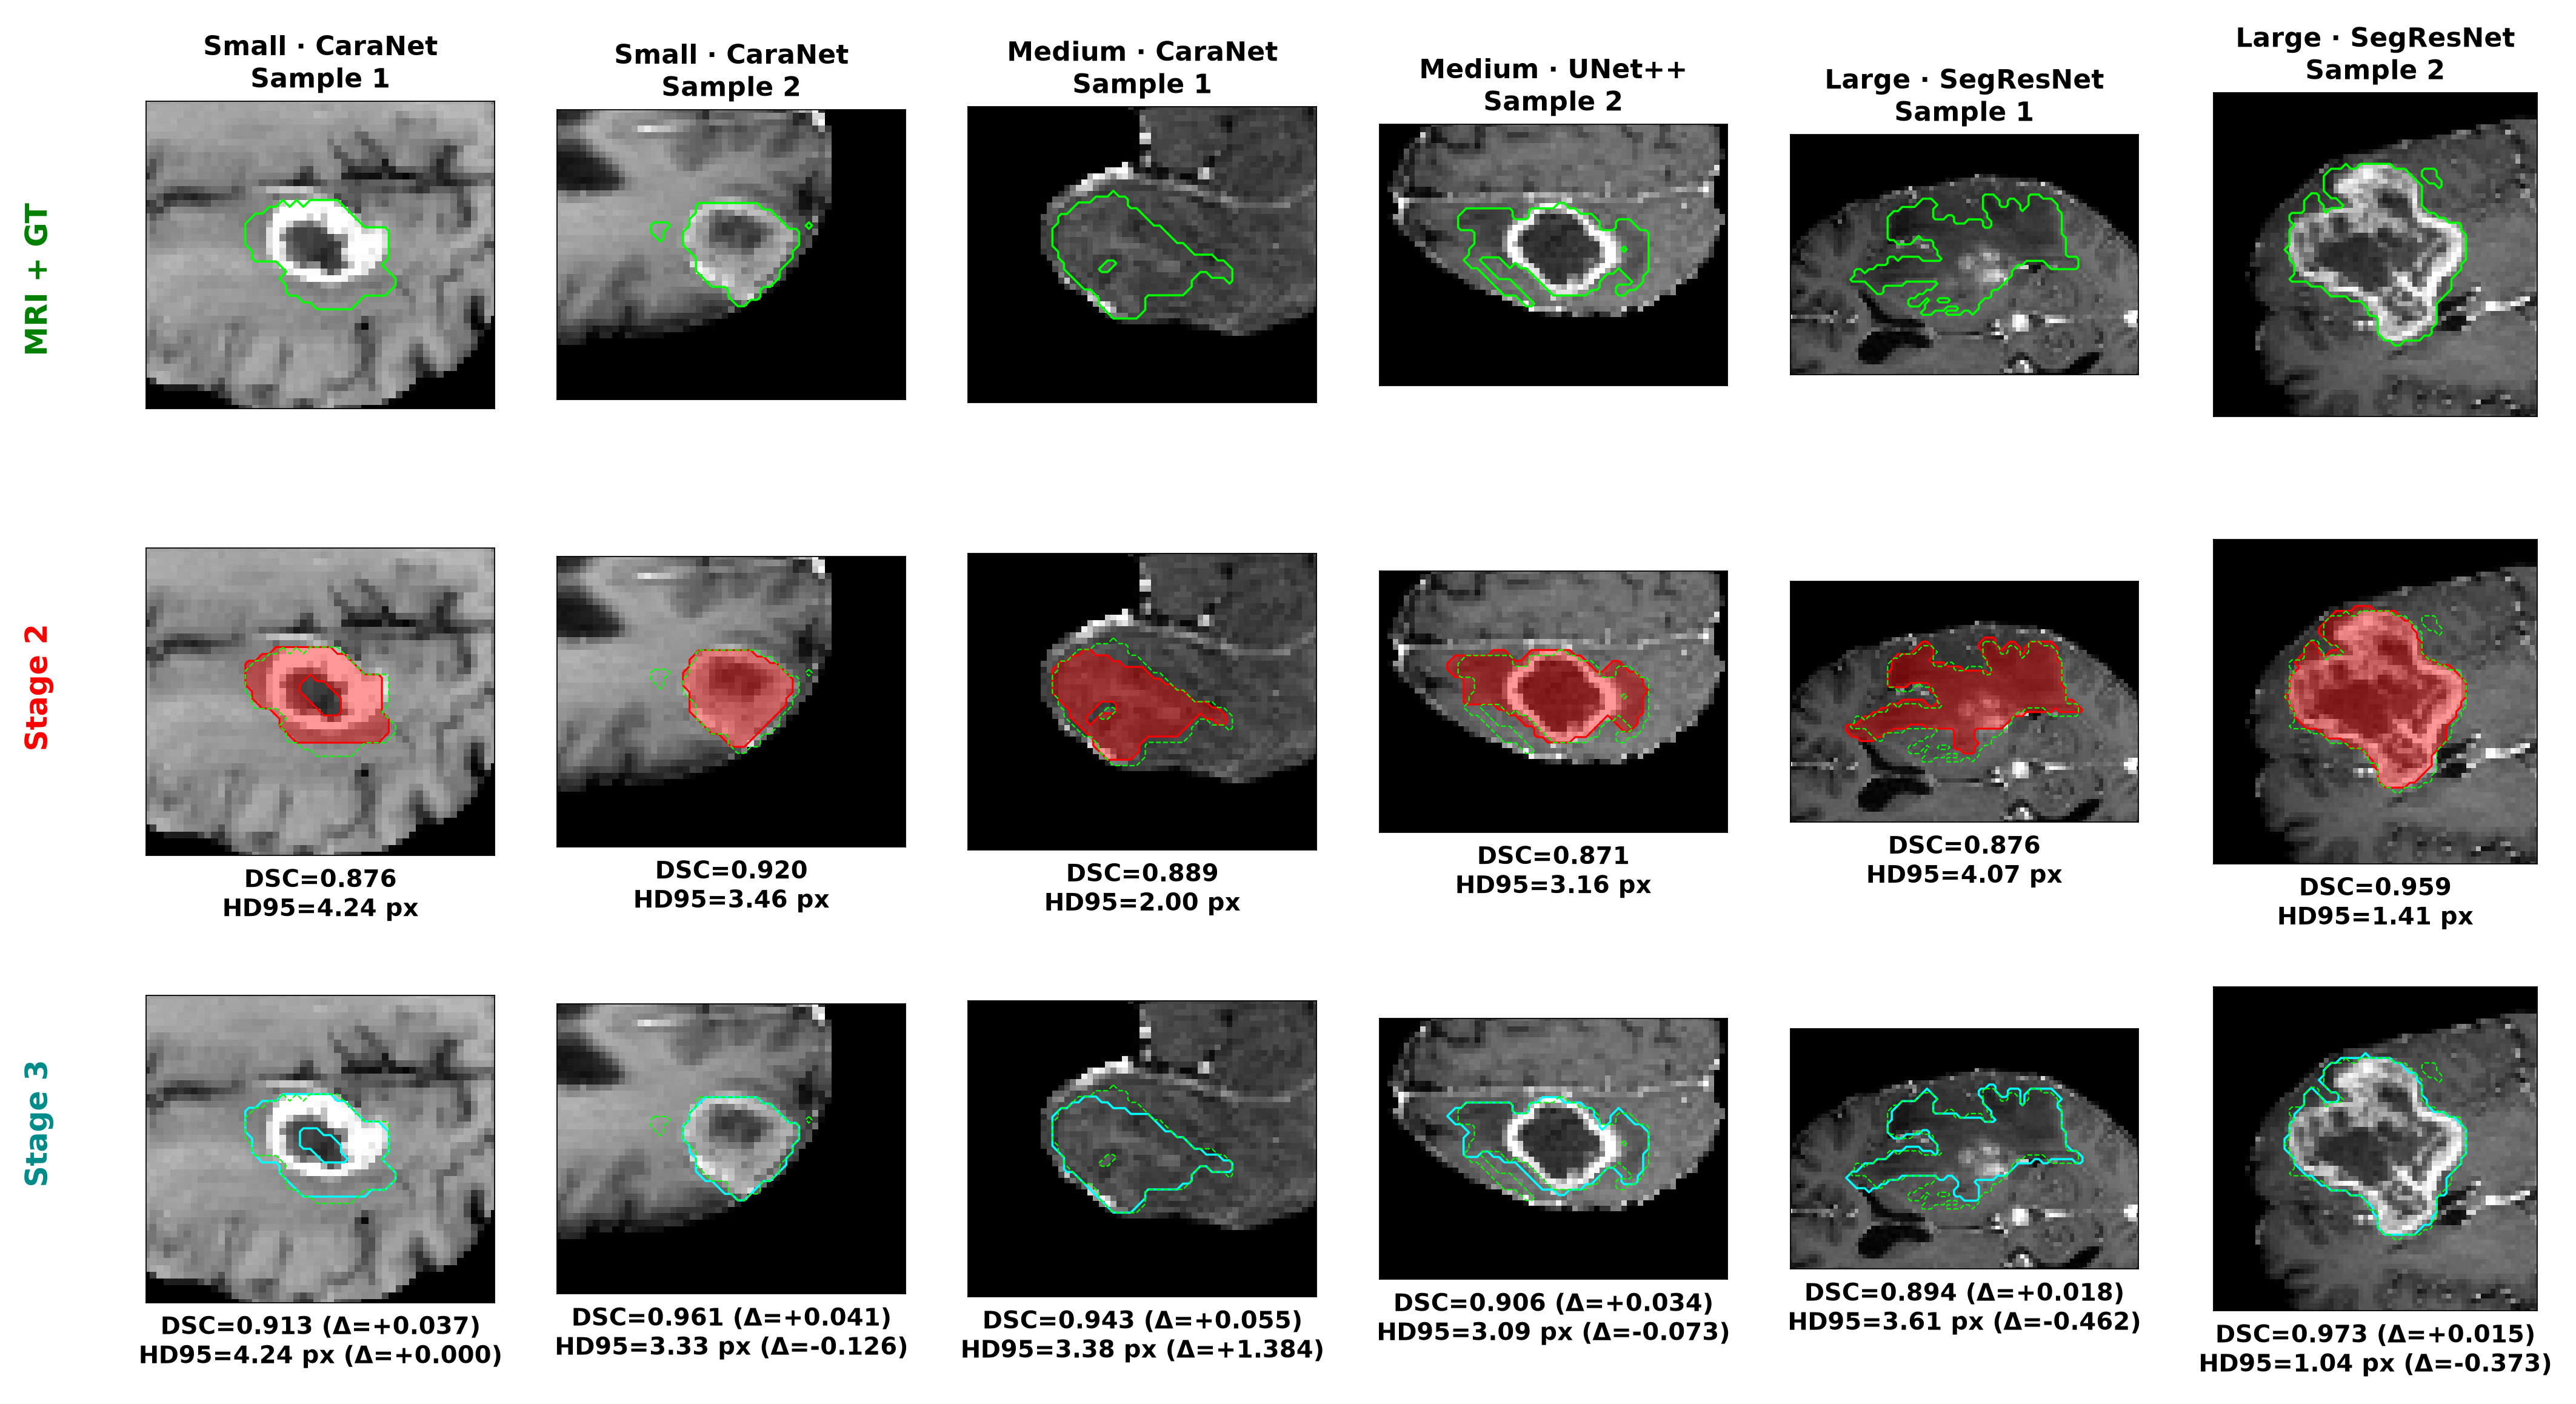
\includegraphics[width=\textwidth]{band_ppo_delta_matched/delta_matched_comparison.png}
\caption{Six slices from unused patients. Top: ground truth (green). Middle: Stage~2 (red). Bottom: boundary-band PPO (cyan). DSC and HD95 under each cell are for that slice.}
\label{fig:delta}
\end{figure}

\subsection{Threshold Reselection Control}
\label{sec:retune}
Stage~2 at the fixed thresholds is biased toward a narrow mask, with precision 0.883 and recall 0.820. To test whether the Table~\ref{tab:locked} gap is only a threshold adjustment, we jointly reselected the three per-size thresholds on the 60 validation patients by patient-mean DSC under classifier routing. The grid is 0.10--0.90 in steps of 0.05, and the connected-component sizes are unchanged. The selected values are 0.45, 0.80, and 0.20 for small, medium, and large, none of which is a grid endpoint. Validation DSC moved from 0.8588 to 0.8650. Those thresholds were applied once to the 851 patients. PPO weights were not changed; they were trained on the fixed-threshold masks.

\begin{table}[t]
\caption{Unused 851 patients. Paired comparison against Stage~2 with reselected thresholds.}
\label{tab:retune}
\centering
\small
\begin{tabular}{lcccc}
\toprule
Area & Fixed Stage~2 & Reselected & PPO & PPO $-$ reselected (95\% CI) \\
\midrule
Overall & 0.8337 & 0.8411 & \textbf{0.8604} & $+0.0193$ (0.0184--0.0202) \\
$<300$ px & 0.7579 & 0.7682 & \textbf{0.7933} & $+0.0251$ (0.0237--0.0265) \\
300--700 px & 0.8700 & 0.8790 & \textbf{0.8952} & $+0.0162$ (0.0154--0.0170) \\
$\geq700$ px & 0.8981 & 0.9014 & \textbf{0.9169} & $+0.0156$ (0.0143--0.0169) \\
\bottomrule
\end{tabular}
\end{table}

Threshold reselection alone has paired difference $+0.0074$ (0.0066--0.0082), about 28\% of the $+0.0267$ in Table~\ref{tab:locked}. The remaining $+0.0193$ is still above the reselected Stage~2, and the interval excludes zero in every range. Reselection raises recall from 0.820 to 0.849 and lowers precision from 0.883 to 0.863. PPO reaches precision 0.892 and recall 0.860, both above the reselected Stage~2. Starting PPO from the reselected masks yields the same overall DSC, 0.8604. The band appears to cover most of the gap between the two thresholds; that fraction was not measured separately.

\subsection{Ablation Study}
\label{sec:retrain}
The weights differ from the 2026-09-30 lock in Table~\ref{tab:locked}. The patient split is unchanged, and only the seed changes, to 42, 7, and 123. Table~\ref{tab:seeds} is the patient mean of tumor-slice DSC. The range of boundary-band PPO DSC across seeds is 0.0023, and the three-seed mean is 0.8609.

\begin{table}[t]
\caption{Retraining on the same split. Patient mean of tumor-slice DSC.}
\label{tab:seeds}
\centering
\begin{tabular}{lccc}
\toprule
Seed & Stage~2 & Band PPO & Large expert, all slices \\
\midrule
42 & 0.8339 & \textbf{0.8597} & 0.8503 \\
7 & 0.8370 & \textbf{0.8620} & 0.8540 \\
123 & 0.8352 & \textbf{0.8609} & 0.8500 \\
\bottomrule
\end{tabular}
\end{table}

Table~\ref{tab:ablate} changes only the inference condition on the seed-42 weights. Rows are the 851-patient mean except the last, which drops the 148 patients shared with the earlier 210-patient pool. Five steps score above one step and above one step of the medium supervised initialization. Radius 0 falls to 0.8427, while three steps, the guard removed, and the two band-width changes stay in 0.8575--0.8601.

\begin{table}[t]
\caption{Seed-42 inference ablation. Patient-mean DSC.}
\label{tab:ablate}
\centering
\begin{tabular}{lc}
\toprule
Condition & DSC \\
\midrule
5-step boundary-band PPO & \textbf{0.8597} \\
1 step & 0.8460 \\
Medium supervised initialization, 1 step & 0.8383 \\
Large expert + boundary-band PPO & 0.8676 \\
Ground-truth-size routing, 5 steps & 0.8698 \\
Radius 0 & 0.8427 \\
3 steps & 0.8589 \\
FLAIR guard off & 0.8575 \\
Radius 4 & 0.8596 \\
Probability band $[0.45,0.55]$ & 0.8597 \\
Probability band $[0.25,0.75]$ & 0.8601 \\
5 steps, 703 patients & 0.8579 \\
\bottomrule
\end{tabular}
\end{table}

Table~\ref{tab:gaps} uses 131{,}905 slices, including empty ones. The false-positive rate is the fraction of slices with tumor-pixel fraction below 0.2\% on which a mask appears. HD95 is the patient mean on slices where Stage~2 and the PPO both have a mask, in millimetres (pixel $\times 1.9$). 3D Dice stacks slices along $z$. A dash means that common-mask HD95 was not computed for the large expert.

\begin{table}[t]
\caption{Empty-slice false positives, common-mask HD95, and 3D Dice.}
\label{tab:gaps}
\centering
\footnotesize
\setlength{\tabcolsep}{4pt}
\begin{tabular}{clccc}
\toprule
Seed & Metric & Stage~2 & Band PPO & Large, all slices \\
\midrule
42 & False positive & 0.567 & \textbf{0.521} & 0.930 \\
42 & HD95 (mm) & 11.536 & \textbf{10.734} & -- \\
42 & 3D Dice & 0.779 & \textbf{0.813} & 0.799 \\
7 & False positive & 0.532 & \textbf{0.497} & 0.821 \\
7 & HD95 (mm) & 10.979 & \textbf{10.351} & -- \\
7 & 3D Dice & 0.786 & \textbf{0.811} & 0.796 \\
123 & False positive & 0.601 & \textbf{0.571} & 0.829 \\
123 & HD95 (mm) & 11.516 & \textbf{10.731} & -- \\
123 & 3D Dice & 0.771 & \textbf{0.809} & 0.759 \\
\bottomrule
\end{tabular}
\end{table}

Table~\ref{tab:unet} is a single U-Net trained for 20 epochs on the same 280 patients, thresholded at 0.5, and evaluated on the 851 patients (50{,}010 tumor slices). The vanilla PPO then edits that mask by a global one-pixel shrink, keep, or expand for 15 steps. The paired patient difference is $-0.0023$ (95\% CI $-0.0029$--$-0.0017$). The size rows have 851, 757, and 408 patients.

\begin{table}[t]
\caption{Single U-Net and a global vanilla PPO. Patient mean on 851 patients.}
\label{tab:unet}
\centering
\small
\setlength{\tabcolsep}{4pt}
\begin{tabular}{lccccc}
\toprule
Method & DSC (95\% CI) & HD95 (px) & Small & Medium & Large \\
\midrule
U-Net & 0.8156 (0.8067--0.8243) & 6.939 & 0.7215 & 0.8758 & 0.8973 \\
Vanilla PPO & 0.8133 (0.8046--0.8220) & 6.955 & 0.7197 & 0.8736 & 0.8939 \\
\bottomrule
\end{tabular}
\end{table}

\section{Conclusion}

TRIO is size classification, size-specific experts, and one boundary-band PPO. On 851 unused patients the patient-mean DSC is 0.8337 before the PPO, at Stage~2, and 0.8604 after five steps of the boundary-band PPO. The paired patient difference $+0.0267$ has 95\% CI $0.0256$--$0.0278$. The difference is largest below 300 pixels, at $+0.0354$, and smallest at 700 pixels or more, at $+0.0188$.

The remaining experiments measure the threshold, retraining, the step count, a single large expert, and a global vanilla PPO. Stage~2 with per-size thresholds reselected on the 60 validation patients scores 0.8411, and its paired difference from the PPO is $+0.0193$ (95\% CI $0.0184$--$0.0202$). Threshold reselection alone accounts for $+0.0074$. Retraining the same split on 2026-10-07 at seeds 42, 7, and 123 keeps boundary-band PPO DSC in 0.8597--0.8620. At seed 42 the five-step PPO scores 0.8597, one step scores 0.8460, one step of the medium supervised initialization scores 0.8383, and the large expert on every slice scores 0.8503. On the same 851 patients a single U-Net scores 0.8156, and a vanilla PPO that shrinks, keeps, or expands the whole mask by one pixel scores 0.8133. At seed 42 the empty-slice false-positive rate falls from 0.567 to 0.521, and 3D Dice after stacking slices rises from 0.779 to 0.813.

\begin{thebibliography}{15}
\bibitem{ronneberger2015}
Ronneberger, O., Fischer, P., Brox, T.: U-Net: Convolutional networks for biomedical image segmentation. In: MICCAI. pp. 234--241 (2015)

\bibitem{zhou2019}
Zhou, Z., Siddiquee, M.M.R., Tajbakhsh, N., Liang, J.: UNet++: Redesigning skip connections to exploit multiscale features in image segmentation. IEEE Trans. Med. Imaging \textbf{39}(6), 1856--1867 (2020)

\bibitem{myronenko2018}
Myronenko, A.: 3D MRI brain tumor segmentation using autoencoder regularization. In: BrainLes (MICCAI). pp. 311--320 (2018)

\bibitem{lou2023}
Lou, A., Guan, S., Loew, M.: CaraNet: Context axial reverse attention network for segmentation of small medical objects. J. Med. Imaging \textbf{10}(1), 014005 (2023)

\bibitem{schulman2017}
Schulman, J., Wolski, F., Dhariwal, P., Radford, A., Klimov, O.: Proximal policy optimization algorithms. arXiv:1707.06347 (2017)

\bibitem{baid2021}
Baid, U., et al.: The RSNA-ASNR-MICCAI BraTS 2021 benchmark on brain tumor segmentation and radiogenomic classification. arXiv:2107.02314 (2021)

\bibitem{liao2020}
Liao, X., Li, W., Xu, Q., Wang, X., Jin, B., Zhang, X., Zheng, Y.: Iteratively-refined interactive 3D medical image segmentation with multi-agent reinforcement learning. In: CVPR. pp. 9394--9402 (2020)

\bibitem{furuta2020}
Furuta, R., Inoue, N., Yamasaki, T.: PixelRL: Fully convolutional reinforcement learning with action-successor representation for image processing. IEEE Trans. Multimedia (2020)

\bibitem{isensee2021}
Isensee, F., Jaeger, P.F., Kohl, S.A.A., Petersen, J., Maier-Hein, K.H.: nnU-Net: a self-configuring method for deep learning-based biomedical image segmentation. Nature Methods \textbf{18}(2), 203--211 (2021)

\bibitem{menze2015}
Menze, B.H., et al.: The Multimodal Brain Tumor Image Segmentation Benchmark (BRATS). IEEE Trans. Med. Imaging \textbf{34}(10), 1993--2024 (2015)

\bibitem{bakas2017}
Bakas, S., et al.: Advancing The Cancer Genome Atlas glioma MRI collections with expert segmentation labels and radiomic features. Scientific Data \textbf{4}, 170117 (2017)

\bibitem{wang2018}
Wang, G., Li, W., Ourselin, S., Vercauteren, T.: Automatic brain tumor segmentation using cascaded anisotropic convolutional neural networks. In: BrainLes (MICCAI). pp. 178--190 (2018)

\bibitem{chen2016}
Chen, H., Qi, X., Yu, L., Heng, P.A.: DCAN: Deep contour-aware networks for accurate gland segmentation. In: CVPR. pp. 2487--2496 (2016)
\end{thebibliography}

\end{document}
